% !TEX TS-program = XeLaTeX
\def \Subject {تمرین حمله به DES}
\def \Course {درس امنیت سیستم های کامپیوتری}
\def \Author {ملیکا محمدی فخار - ستاره باباجانی}
\def \StudentNumber {99522086-99521109}

\documentclass[11pt]{article}

\usepackage[]{algorithm2e}
\usepackage{cite}
\usepackage{calc}
\usepackage{minted}
\usepackage{fancyhdr}
\usepackage{lipsum}
\usepackage{color}
\usepackage{ragged2e}
\usepackage[inline]{enumitem}
\usepackage[dvipsnames]{xcolor}
\usepackage{graphicx}
\usepackage{wrapfig}
\usepackage{float}
\usepackage{tabu}
\usepackage{hyperref}
\usepackage{xepersian}
\usepackage{minted}

\settextfont[BoldFont={XB Yas Bd}, ItalicFont={XB Yas It}, BoldItalicFont={XB Yas BdIt}, Extension = .ttf]{XB Yas}

\fancyhead[L]{
\includegraphics[scale = 0.07]{images/IUST_logo_color.png}}
\fancyhead[R]{\large \Course}
\fancyhead[C]{\Large \Subject}
\renewcommand{\headrulewidth}{0.5mm}
\pagestyle{fancy}
\setlength{\headheight}{28pt}

\setminted{
    frame=lines,
    framesep=2mm,
    baselinestretch=1.0,
    xrightmargin=0in,
    xleftmargin=0in,
    fontsize=\footnotesize,
    linenos=false
}

\newcommand{\grayBox}[1]{\colorbox{gray!10}{\lr{\texttt{#1}}}}
\newcommand{\grayLBox}[1]{\fbox{\grayBox{\parbox{11.8 cm}{#1}}}}

\makeatletter
\newcommand{\chapterauthor}[1]{%
    {\parindent0pt\vspace*{-25pt}%
        \linespread{1.1}\large\scshape#1%
        \par\nobreak\vspace*{35pt}}
    \@afterheading%
}
\makeatother

\title{
    
\includegraphics[width=0.5\linewidth]{images/IUST_logo_color.png} \\
    دانشکده مهندسی کامپیوتر \\
}

\author{
    \Course \\ \vspace{0.5cm}
    \Subject \\ \vspace{0.5cm}
    \Author \\ \vspace{0.5cm}
    \StudentNumber \\ \vspace{0.5cm}
    استاد درس: دکتر ابوالفضل دیانت
}
\date{بهار 1403}

\begin{document}
    \maketitle
    \newpage
\section*{سوال اول: حمله تفاضلی به DES}

یکی از مهم‌ترین حملات به DES، حمله تفاضلی است که توسط Eli Biham و Adi Shamir در دهه 1990 مطرح شد. در مورد این حمله تحقیق کنید و نحوه این حمله را با یک مثال ساده شده DES بیان کنید. مثلا با DES سه دور یا شش دور.

\subsection*{پاسخ: حمله تفاضلی به DES}

حمله تفاضلی یک تکنیک رمزنگاری است که به تحلیل تغییرات در ورودی و خروجی یک الگوریتم رمزنگاری پرداخته و از تفاوت‌های مشاهده شده برای کشف کلید مخفی استفاده می‌کند. در DES این حمله با استفاده از تفاوت‌های ورودی و خروجی در چندین دور از الگوریتم، سعی در یافتن کلید دارد.

به عنوان مثال، فرض کنید دو متن ساده $P$ و $P'$ که در یک بیت تفاوت دارند (یعنی $\Delta P = P \oplus P'$) به الگوریتم DES داده می‌شوند و متن‌های رمز شده $C$ و $C'$ تولید می‌شوند. تفاوت متن رمز شده $\Delta C = C \oplus C'$ است.

حمله کننده با تحلیل تفاوت‌های ورودی و خروجی در چندین دور DES و استفاده از جدول‌های تفاوتی برای S-boxها می‌تواند بخشی از کلید مخفی را پیدا کند.

در یک DES سه دور، فرض کنید تفاوت ورودی $\Delta P$ را می‌دانیم. با تحلیل تفاوت‌ها در خروجی هر S-box و استفاده از خواص آن‌ها، می‌توانیم تفاوت در خروجی هر دور را محاسبه کنیم و از این اطلاعات برای حدس زدن کلید استفاده کنیم.

\section*{سوال دوم: الگوریتم AES }
\subsection*{نکات کلیدی}
\begin{itemize}
    \item \textbf{الگوریتم کلید متقارن}: AES از یک کلید برای هر دو فرآیند رمزگذاری و رمزگشایی استفاده می‌کند. این به این معنی است که هم فرستنده و هم گیرنده باید به همان کلید دسترسی داشته باشند.
    \item \textbf{رمز بلاکی}: AES داده‌ها را در بلاک‌های با اندازه ثابت رمزگذاری می‌کند. اندازه استاندارد بلاک 128 بیت است، اما می‌تواند بلاک‌هایی با اندازه 192 و 256 بیت را نیز پردازش کند.
\end{itemize}

\subsection*{مراحل الگوریتم AES}

\subsubsection*{گسترش کلید}
کلید اولیه داده شده به چندین کلید دوری با استفاده از برنامه کلید AES گسترش می‌یابد. تعداد دورها بستگی به طول کلید دارد:
\begin{itemize}
    \item 10 دور برای کلیدهای 128 بیتی
    \item 12 دور برای کلیدهای 192 بیتی
    \item 14 دور برای کلیدهای 256 بیتی
\end{itemize}

\subsubsection*{دور اولیه}
\begin{itemize}
    \item \textbf{AddRoundKey}: هر بایت از بلاک با یک بایت از کلید دوری با استفاده از عملیات XOR ترکیب می‌شود.
\end{itemize}

\subsubsection*{دورهای اصلی}
(9، 11، یا 13 بار بسته به اندازه کلید تکرار می‌شود):
\begin{itemize}
    \item \textbf{SubBytes}: هر بایت از بلاک با بایت معادل در یک جدول جایگزینی ثابت (S-box) جایگزین می‌شود.
    \item \textbf{ShiftRows}: ردیف‌های بلاک به صورت چرخشی جابجا می‌شوند. هر ردیف به میزان متفاوتی جابجا می‌شود.
    \item \textbf{MixColumns}: ستون‌های بلاک با ضرب در یک چندجمله‌ای ثابت در میدان گالوا مخلوط می‌شوند.
    \item \textbf{AddRoundKey}: بلاک جاری با کلید دوری با استفاده از XOR ترکیب می‌شود.
\end{itemize}

\subsubsection*{دور نهایی}
(همانند دورهای اصلی اما بدون مرحله MixColumns):
\begin{itemize}
    \item SubBytes
    \item ShiftRows
    \item AddRoundKey
\end{itemize}

\subsection*{رمزگشایی}
فرآیند رمزگشایی معکوس رمزگذاری است. شامل همان مراحل است اما به ترتیب معکوس و با عملیات معکوس:
\begin{itemize}
    \item Inverse SubBytes
    \item Inverse ShiftRows
    \item Inverse MixColumns
    \item AddRoundKey
\end{itemize}

\section*{کد}

\subsection*{تحلیل کد}

این کد پایتون از کتابخانه \texttt{PyCryptodome} برای رمزنگاری و رمزگشایی متن با استفاده از الگوریتم AES در حالت CBC استفاده می‌کند. کد شامل مراحل زیر است:


\begin{itemize}
    \item وارد کردن کتابخانه‌ها
    \item تولید کلید و داده ورودی
    \item رمزنگاری
    \item چاپ داده‌های رمزنگاری شده
    \item رمزگشایی
    \item نتایج
\end{itemize}


\begin{figure}
    \centering
    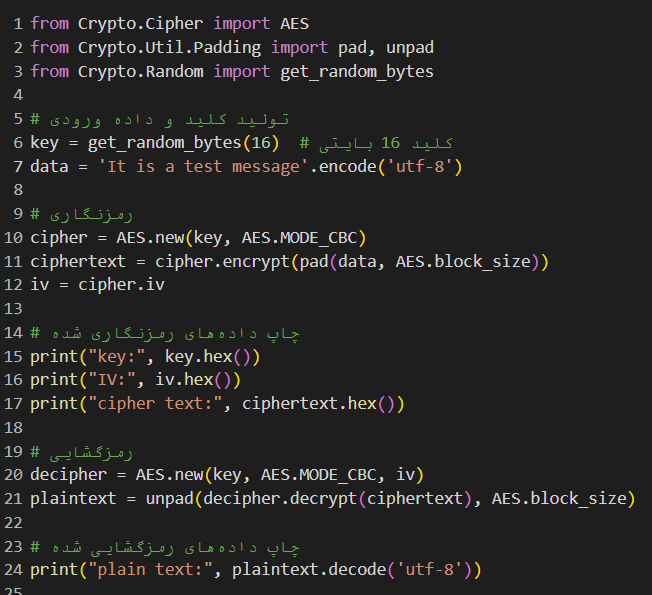
\includegraphics[width=1\linewidth]{Annotation 2024-05-29 184413.png}
    \caption{کد زده شده}
    \label{fig:enter-label}
\end{figure}

\begin{figure}
    \centering
    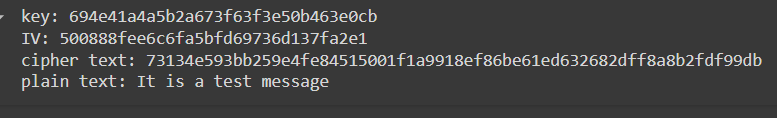
\includegraphics[width=1.2\linewidth]{Annotation 2024-05-29 184428.png}
    \caption{خروجی کد}
    \label{fig:enter-label}
\end{figure}



\end{document}